\chapter{Models \label{ch:models}}

In this chapter, we describe the specific models that we use for analyzing fMRI data and tracking a disease epidemic. We also describe models that we simulate data from in order to compare the performance of different particle filtering algorithms. All of these models fall into a general class of models called \emph{state-space models}. In Section \ref{sec:ss}, we describe state-space models in general. In Section \ref{sec:epid}, we describe the model used for tracking a disease epidemic. In Section \ref{sec:dlm}, we describe a subclass of state-space models called \emph{dynamic linear models} that we use to model fMRI data. In Section \ref{sec:sequential}, we describe sequential estimation of states and unknown fixed parameters in state-space models in general and give explicit solutions for special cases.

\section{State-space models \label{sec:ss}}

State-space models are a general class of statistical models used for analysis of dynamic data.  They are constructed using an observation equation, $y_t \sim p_{y,t}(y_t|x_t,\theta)$, and a state evolution equation, $x_t \sim p_{x,t}(x_t|x_{t-1},\theta)$, where $y_t$ is the observed response, $x_t$ is a latent, dynamic state, the subscript $t$ is a time index, and $\theta$ is an unknown fixed parameter, all of which could be vectors. The $y_t$'s are assumed independent given $x_t$ and $\theta$, and the $x_t$'s are assumed independent given $x_{t-1}$ and $\theta$ (see Figure \ref{fig:ssdraw}). The distributions $p_{y,t}$ and $p_{x,t}$ are assumed known conditional on the values of $\theta$ and $x_t$ in the observation equation and $\theta$ and $x_{t-1}$ in the evolution equation. Depending on whether the observations and the states are continuous or discrete, the distributions themselves may be continuous or discrete. The distributions are typically assumed to only vary with $x_t$ and $\theta$, and therefore the $t$ subscript is dropped. For simplicity, we also drop the $x$ and $y$ subscript and instead let the arguments make clear which distribution we are referring to. Thus, the general state-space model is
\begin{align}
y_t &\sim p(y_t|x_t,\theta) \label{eqn:obs} \\
x_t &\sim p(x_t|x_{t-1},\theta). \label{eqn:state}
\end{align}
A fully specified Bayesian model is obtained by also specifying the prior $p(x_0,\theta)$.

\begin{figure}[ht]
\centering
\caption{Dependence structure of state-space models} \label{fig:ssdraw}
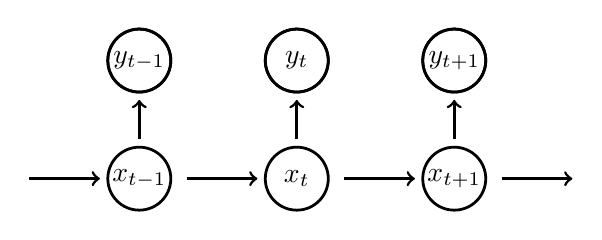
\begin{tikzpicture}[line width=1pt]
\foreach \x in {1,...,3} \draw (3+2*\x,0) circle (0.4cm);
\foreach \x in {1,...,3} \draw (3+2*\x,1.5) circle (0.4cm);
\foreach \x in {1,...,3} \draw (3+2*\x,1.5) circle (0.4cm);
\foreach \x in {1,...,3} \draw [<-] (3+2*\x, 1) -- (3+2*\x,.5);
\foreach \x in {1,...,4} \draw [->] (3+2*\x-1.4, 0) -- (3+2*\x-.5,0);
\draw (3+2*1,0) node {$x_{t-1}$};
\draw (3+2*2,0) node {$x_{t}$};
\draw (3+2*3,0) node {$x_{t+1}$};
\draw (3+2*1,1.5) node {$y_{t-1}$};
\draw (3+2*2,1.5) node {$y_{t}$};
\draw (3+2*3,1.5) node {$y_{t+1}$};
\end{tikzpicture}
\end{figure}

Equations \eqref{eqn:obs} and \eqref{eqn:state} describe a very general class of models, including non-Markovian structures and models where the dimension of $x_t$ does not remain constant with respect to $t$. For instance, we could describe a process where $x_t$ depends on the entire history of states up to $t$ by letting $x_{t-1} = (x^*_1, x^*_2, \ldots, x^*_{t-1})'$ and defining $x_t = (x_{t-1}, x^*_t)'$, where $x^*_t$ is the new state generated at time $t$. In addition, the form of equations \eqref{eqn:obs} and \eqref{eqn:state} could be linear or nonlinear with respect to $x_t$ or $\theta$. For example, in Section \ref{sec:epid}, we describe a state-space model of a disease outbreak that is nonlinear in the observation equation with respect to $x_t$ and nonlinear in the state equation with respect to $\theta$. In Chapter \ref{ch:epid}, we compare the performance of several particle filtering algorithms using data simulated from this model.

Special cases of state-space models include hidden Markov models \citep{cappe:2005:inference}, where $x_t$ has discrete support, and dynamic linear models (DLMs) \citep{West:Harr:baye:1997, petris:camp:2009:dynamic}, where each distribution is Gaussian whose mean is a linear function of the states and whose variance does not depend on the mean. A simple form of a DLM, known as a first-order DLM or local-level model, is described in Section \ref{sec:dlm:ll} and used in Chapter \ref{ch:comp} to compare several particle filtering algorithms in terms of their ability to estimate $p(y_{1:t})$, the \emph{marginal likelihood} of the data. In Chapter \ref{ch:fmri}, DLM representations of regression models with autocorrelated errors are used to analyze fMRI data. We describe DLMs in more detail in Section \ref{sec:dlm}.

\section{Model for tracking an epidemic \label{sec:epid}}

In this section, we describe a state-space model of an epidemic in which we track the proportion of the population that is susceptible ($s_t$), infectious ($i_t$), and recovered ($r_t$), i.e. no longer able to be infected, at time $t$. Mathematically, $s_t$, $i_t$, and $r_t$ are all nonnegative and $s_t + i_t + r_t = 1$ for all $t$. When monitoring an epidemic, the true $s_t$, $i_t$ and $r_t$ are unknown and regarded as hidden states of the model, and the observed data are gathered via syndromic surveillance. In our state-space model of an epidemic, the observation equation specifies how the observed data depend on the state of the epidemic and the state equation describes how the epidemic evolves over time.

\subsection{SIR model \label{sec:epid:state}}

First, we describe the state equation. Let $x_t = (s_t,i_t)'$ denote the state of the epidemic at time $t$ (by definition $r_t=1-s_t-i_t$ and hence $r_t$ is not needed in the state vector). Initially, we consider a compartmental model - or SIR model - of disease transmission that is governed by three parameters:

\begin{itemize}
\item $\beta$, the contact rate for the spread of illness,
\item $\gamma$, the recovery time from infection (i.e. the reciprocal of the average infectious period), and
\item $\nu$, the mixing intensity of the population.
\end{itemize}

\noindent $\beta$, $\gamma$, and $\nu$ are each restricted to be nonnegative. Define $\theta = (\beta,\gamma,\nu)'$ to be the vector of unknown parameters in our model and let $P$ be the size of the population. Then, we describe the evolution of the epidemic from time $t$ to $t + 1$ by

\begin{equation}
x_{t+1}\left|x_t,\theta\right. \sim \mbox{N}_\Omega\left(f(x_t,\theta),Q(\theta)\right), \label{eqn:epid:state}
\end{equation}
\noindent where
\[
f(x_t,\theta) = \left(
\begin{array}{c}
s_t - \beta i_ts^\nu_t \phantom{- \gamma i_t}\,\, \\
i_t +  \beta i_ts^\nu_t - \gamma i_t
\end{array}
\right)
\qquad
Q(\theta) = \frac{\beta}{P^2} \left(
\begin{array}{ccccc}
1 & -1 \\
-1 & 1 + \gamma/\beta
\end{array}
\right)
\]

\noindent and $\Omega = \{(s_t,i_t): s_t \ge 0, i_t \ge 0, s_t + i_t \le 1\}$.

In equation \eqref{eqn:epid:state}, $Q(\theta)$ is determined by calculating the variances and covariance of $s_{t+1}$ and $i_{t+1}$ in the discrete time approximation of a modified SIR model with stochastic fluctuations \citep{herwaarden1995stochepid, dangerfield2009stochepid, anderson2004sars}, given by
\begin{align}
s_{t+1} &= s_t - \beta i_ts^\nu_t + \epsilon_\beta \label{eqn:disc:sus} \\
i_{t+1} &= i_t + \beta i_ts^\nu_t - \gamma i_t - \epsilon_\beta + \epsilon_\gamma, \label{eqn:disc:inf}
\end{align}
where $\epsilon_\beta$ and $\epsilon_\gamma$ are random components with $\epsilon_\beta \sim \mbox{N}(0, \sqrt{\beta} / P)$ and $\epsilon_\gamma \sim \mbox{N}(0, \sqrt{\gamma} / P)$. The variances of these terms come from a scaling law for stochastic fluctuations in a dynamical system generated by random contacts among the population \citep{ovaskainen2010extinction, herwaarden1995stochepid, dangerfield2009stochepid, skvortsov2012monitoring}.

The \emph{basic reproductive number}, $R_0 = \beta / \gamma$, is the average number of people infected by one sick person in a population where everyone is susceptible \citep{heff2005repratio}. If $R_0 > 1$, then an epidemic can occur. In many cases, prior information about $R_0$ for a specific type of infection is more readily available than prior knowledge about $\beta$ or $\gamma$ individually.

The mixing parameter $\nu$ describes the heterogeneity of social interactions within the population, where $\nu = 1$ corresponds to a population with homogenous mixing, i.e. an infectious person is equally likely to infect any susceptible, and $\nu = 0$ corresponds to a population with no social interaction. Values of $\nu > 1$ represent populations with heterogenous mixing, i.e. an individual is more likely to interact with some people more than others, leading to less severe epidemics than those that would occur in homogenous populations for a fixed $R_0$ \citep{stroud2006powerlaw, novozhilov2008hetero}.

\subsection{Syndromic surveillance data \label{sec:epid:obs}}

The observed data from syndromic surveillance are positive real numbers related to counts of emergency room visits, prescription sales, or calls to a hotline, for example, and we can observe data from these different streams/sources asynchronously in time. That is, at any time $t$, we can observe data from any subset of the streams (or possibly none of them). Let $y_{l,t}>0$ represent data coming from stream $l$ at time $t$, where $l = 1,2,\ldots,L$ and $t = 1,2,\ldots,T$. We model the log of the observations by
\begin{equation}
\log y_{l,t} \sim \mbox{N}\left(b_li_t^{\varsigma_l} + \eta_l,\sigma_l^2\right), \label{eqn:epid:obs}
\end{equation}
where $b_l$, $\varsigma_l$, and $\sigma_l$ are nonnegative constants \citep{skvortsov2012monitoring} and $\eta_l$ is a real number that determines the baseline level of incoming syndromic data from stream $l$.

The form of the mean of $\log y_{l,t}$ in equation \eqref{eqn:epid:obs} is derived from a simplification of the power-law relationship, described in \citet{skvortsov2012monitoring} and \citet{Gins:Mohe:Pate:Bram:Smol:Bril:dete:2009}, between syndromic observations and the proportion of the population that is infectious, where $b_l$ is a multiplicative constant that depends on the syndromic data source, $\varsigma_l$ is the power-law exponent, and $\sigma_l$ is the standard deviation term that determines the magnitude of random fluctuations in the syndromic observations from stream $l$. In Chapter \ref{ch:epid}, we first consider the case where $b_l$, $\varsigma_l$, $\sigma_l$, and $\eta_l$ are assumed known, as in \citep{skvortsov2012monitoring}, but then relax that assumption in an extended analysis.

Having formulated the data-generating model, we define $y_t = (y_{1,t},\ldots,y_{L,t})'$ and specify $p(y_t|x_t,\theta)$, i.e. the likelihood of an observation $y_t$ given $x_t$ and $\theta$, according to $\mbox{LN}(\mu_t,\Sigma_t)$, where $\mu_t$ is an $L$-length vector with element $l$ equal to $b_li_t^{\varsigma_l} + \eta_l$ and $\Sigma_t$ is an $L \times L$ diagonal matrix with the $l^{\mbox{th}}$ diagonal equal to $\sigma_l^2$. Elements of $y_t$ may be missing, in which case the dimensions of $y_t$, $\mu_t$, and $\Sigma_t$ shrink by the number of missing elements. If all elements of $y_t$ are empty (i.e. if no syndromic data are observed at time $t$), then $p(x_t,\theta|y_{1:t})=p(x_{t-1},\theta|y_{1:t-1})$.

Lastly, we specify the full Bayesian model through $p(x_0, \theta)$, the joint prior distribution of the initial state of the epidemic and the fixed parameters. We use a prior of the form $p(x_0,\theta) = p(\theta)p(s_0,i_0)$, where $p(s_0,i_0)$ is specified according to
\begin{equation}
i_0 \sim \mbox{N}_{[0,1]}(0.002,0.0005^2) \quad s_0 = 1 - i_0. \label{eqn:epid:prior:state}
\end{equation}
In Chapter \ref{ch:epid} we explore the sensitivity of estimation using particle filtering to different choices for $p(\theta)$.

\section{Dynamic linear models (DLMs) \label{sec:dlm}}

In this section, we describe DLMs in general and detail specific DLMs analyzed in Chapters \ref{ch:comp} and \ref{ch:fmri}. The general form of a DLM is represented as a state space model with observation and state equations given by
\begin{align}
y_t &= F_tx_t + v_t \label{eqn:dlm:obs} \\
x_t &= G_tx_{t-1} + w_t. \label{eqn:dlm:state}
\end{align}
Here, $y_t$ is a $q \times 1$ observation vector, $x_t$ is a $p \times 1$ state vector, and $v_t$ and $w_t$ are independent and identically distributed (iid) Gaussian random variables with mean equal to the zero vector (of length $q$ for $v_t$ and length $p$ for $w_t$) and covariance matrices $V_t$ ($q \times q$) and $W_t$ ($p \times p$), respectively. We also assume $v_t$ and $w_{t'}$ independent for all $t$ and $t'$. $F_t$ is a $q \times p$ matrix that defines the linear dependence between $y_t$ and $x_t$ in the observation equation; $G_t$ is a $p \times p$ matrix that does so for $x_t$ and $x_{t-1}$ in the state equation. Lastly, we specify the full Bayesian DLM by defining the distribution of the prior state according to $x_0 \sim \mbox{N}(m_0, C_0)$, where $m_0$ is a $p \times 1$ vector and $C_0$ is a $p \times p$ matrix. The matrices $V_t$, $W_t$, $F_t$, and $G_t$ are allowed to vary with time, and any or all of $V_t$, $W_t$, $F_t$, $G_t$, and $C_0$ could possibly contain unknown parameters.

All DLMs discussed in chapters \ref{ch:comp} and \ref{ch:fmri} assume univariate observations, i.e. $y_t$ is a scalar and $q = 1$. In addition, we assume $G_t$, $V_t$, and $W_t$ are time invariant, and so the subscript $t$ is omitted. Some DLMs we consider have time-invariant $F_t$, e.g. the local level DLM featured in Chapter \ref{ch:comp} and the dynamic intercept model discussed in Chapter \ref{ch:fmri}, while others such as the dynamic slope model featured in Chapter \ref{ch:fmri} incorporate time-varying $F_t$. Lastly, all DLMs we consider assume $F_t$ is known, while $G$, $V$, and $W$ may contain unknown parameters. We provide an overview of these DLMs in sections \ref{sec:dlm:ll} through \ref{sec:dlm:arwn}.

\subsection{First-order DLM with common variance factor \label{sec:dlm:ll}}

The first-order DLM -- or local level model -- for univariate $y_t$ and $x_t$ is specified by setting $F_t = G = 1$ for all $t$. Note that, in this case, $q = p = 1$ and both $V$ and $W$ are $1 \times 1$ matrices. We also assume that the observation and state variance share an unknown factor, $\theta$, and that the \emph{signal-to-noise ratio}, defined as $\lambda = W / V$, is known. Specifically, we have the following model:
\begin{align}
y_t &\sim \mbox{N}(x_t, \theta) \label{eqn:ll:obs} \\
x_t &\sim \mbox{N}(x_{t-1}, \theta\lambda) \label{eqn:ll:state}
\end{align}
with prior distribution $p(x_0, \theta)$ specified by
\begin{equation}
x_0|\theta \sim \mbox{N}(0, \theta) \quad \theta \sim \mbox{IG}(a_0,b_0), \label{eqn:ll:prior}
\end{equation}
where the hyperparameters $a_0$ and $b_0$ are known.

\subsection{Regression with ARMA errors \label{sec:dlm:arma}}

A DLM is convenient for representing a linear regression model with autocorrelated errors. To do so, we introduce known covariates and unknown regression coefficients into the model, i.e.
\begin{align}
y_t &= U_t\beta + F_tx_t + v_t \label{eqn:dlm:reg:obs} \\
x_t &= Gx_{t-1} + w_t, \label{eqn:dlm:reg:state}
\end{align}
where $U_t$ is a known $q$ by $d$ matrix and $\beta$ is an unknown $d$ by $1$ vector. A regression model could be specified without introducing $U_t$ and $\beta$ and instead incorporating $U_t$ inside of $F_t$ and $\beta$ as part of $x_t$. However, we write the model as in equations \eqref{eqn:dlm:reg:obs} and \eqref{eqn:dlm:reg:state} to make the separation of fixed regression coefficients and the dynamic state explicit.

In Chapter \ref{ch:fmri}, we consider regression models for univariate $y_t$ with autoregressive-moving average (ARMA) error structure, i.e. models of the form given in equations \eqref{eqn:dlm:reg:obs} and \eqref{eqn:dlm:reg:state} with $q = 1$ and $x_t$ following a zero-mean $\mbox{ARMA}(P, Q)$ stochastic process \citep{shum:stof:2006:timeseries}, where $P$ and $Q$ are the orders of the autoregressive (AR) and moving average (MA) components, respectively. In these models, $x_t = (x_{t,1} ,x_{t,2}, \ldots, x_{t,m})'$ is an $m$-dimensional vector with $m = \mbox{max}(P,Q+1)$, $F_t$ is a time-invariant $m \times 1$ vector with first element equal to 1 and the rest 0, $V = 0$ (a $1 \times 1$ matrix), $G$ is an $m \times m$ matrix that takes the form
\[
G = \left(
 \begin{array}{ccccc}
 \phi_1 & \vdots \\
 \phi_2 & \vdots \\
 \phi_3 & \vdots && I_{m-1} \\
 \vdots & \vdots \\
 \cdots & \cdots & \cdots & \cdots & \cdots \\
 \phi_m &\vdots & 0 & \cdots & 0
 \end{array}
\right),
\]
and $W = \sigma^2ee'$ with $e = (1, \gamma_1, \ldots, \gamma_m)'$. We let $\theta = (\beta', \phi', \gamma', \sigma^2)'$ represent the unknown parameters of the model, where $\phi = (\phi_1,\phi_2,\ldots,\phi_P)'$ and $\gamma = (\gamma_1,\gamma_2,\ldots,\gamma_Q)'$ are the coefficients of the AR and MA components, respectively, and $\sigma^2$ is the unknown variance of the ARMA innovations. We adopt the convention that $\phi_s = 0$ for $s > P$ and $\gamma_r = 0$ for $r > Q$. Multiplying out the state equation and successively back-substituting the components of $x_t$ \cite[see Sec 3.2.5,][]{petris:camp:2009:dynamic} yields the more familiar form of a regression model with ARMA errors, given by
\begin{equation}
y_t = U_t\beta + \phi_1x_{t-1,1} + \phi_2x_{t-2,1} + \cdots + \phi_Px_{t-P,1} + \gamma_1\epsilon_{t-1} + \gamma_2\epsilon_{t-2} + \cdots + \gamma_Q\epsilon_{t-Q}, \label{eqn:arma}
\end{equation}
where $\epsilon_t \stackrel{iid}{\sim} \mbox{N}(0,\sigma^2)$. Note that only the first element of the state vector plays a role in equation \eqref{eqn:arma}.

It is often desired that constraints be imposed on $\phi$ and $\gamma$ such that the ARMA process is stationary and invertible. Stationarity ensures that the long term behavior of $x_t$ is predictable and invertibility ensures that current and future states do not depend on the distant past \citep{shum:stof:2006:timeseries}. We require that roots of the AR polynomial
\begin{equation}
\phi(z) = 1 - \phi_1z - \phi_2z^2 - \cdots - \phi_Pz^P \label{eqn:arpoly}
\end{equation}
lie outside of the unit circle in the complex plane to ensure stationarity. To ensure invertibility, we impose the same constraint on the MA polynomial, given by
\begin{equation}
\gamma(z) = 1 + \gamma_1z + \gamma_2z^2 + \cdots + \gamma_Pz^Q. \label{eqn:mapoly}
\end{equation}
In Chapter \ref{ch:fmri}, we impose these constraints when fitting regression models with ARMA errors to fMRI data using maximum likelihood estimation.

In a Bayesian context, these models are completely specified by defining the prior distribution $p(x_0, \theta)$, where the initial state, $x_0$, consists of the presample errors. It is often desired that $x_0$ come from the stationary distribution of the ARMA process, given by
\begin{equation}
x_0|\theta \sim \mbox{N}(0, \sigma^2\Omega), \label{eqn:arma:prior}
\end{equation}
where $\mbox{vec}(\Omega) = (I_m - G\otimes G)^{-1} \mbox{vec}(ee')$ and $\phi$ is restricted to the region of stationarity. For a Bayesian treatment of unknown parameters in regression models with stationary and invertible ARMA errors, we refer the reader to \citet{chib:greenberg:1994:arma}.

\subsection{Dynamic regression \label{sec:dlm:arwn}}

The regression model with ARMA errors described in Section \ref{sec:dlm:arma} is represented as a DLM by setting the observation variance $V$ in equation \eqref{eqn:dlm:reg:obs} equal to 0 and completely specifying the error structure through the state equation. By instead letting $V > 0$, we can add an additional layer of variance to the model that represents observation or measurement noise. Furthermore, we can introduce additional structure into the errors through $F_t$. For example, consider a simple linear regression model with an intercept and a slope given by $\beta_0$ and $\beta_1$, respectively, and errors that follow an AR(1) plus white noise (AR(1)+WN) process, i.e.
\begin{align}
y_t &= \beta_0 + \beta_1u_t + x_t + v_t \label{eqn:arwn:obs} \\
x_t &= \phi x_{t-1} + w_t, \label{eqn:arwn:state}
\end{align}
where $u_t$ is a known explanatory variable, $v_t \stackrel{iid}{\sim} \mbox{N}(0, \sigma^2_m) \perp w_t \stackrel{iid}{\sim} \mbox{N}(0, \sigma^2_s)$, and $\theta = (\beta_0,\beta_1,\phi,\sigma^2_s,\sigma^2_m)'$ represents the unknown parameters in the model. Here, $\phi$ is the lag-1 coefficient of the AR process (note the subscript `1' is removed since there is only 1 AR coefficient), $\sigma^2_m$ is the observation variance, and $\sigma^2_s$ is the state variance, or more precisely the variance of the innovations of the AR(1) process for the state. We will refer to this parameter as the \emph{white noise variance} for the state, since the actual variance of the state is $\sigma^2_s / (1 - \phi^2)$ and $\sigma^2_s$ represents the variance of $w_t$, or the ``white noise'' component of the AR(1) process.

Reexpressing equation \eqref{eqn:arwn:obs} as
\begin{equation}
y_t = (\beta_0 + x_t) + \beta_1u_t + v_t \label{eqn:arwn:dynint}
\end{equation}
shows that we can interpret this model as a \emph{dynamic intercept model}, i.e. a simple linear regression model with an intercept that changes over time according to an AR(1) process. We can represent a dynamic intercept model as a DLM defined by equations \eqref{eqn:dlm:reg:obs} and \eqref{eqn:dlm:reg:state} where $U_t = (1, u_t)$, $\beta = (\beta_0, \beta_1)'$, $F_t = 1$ for all $t$, $V = \sigma^2_m$, $G = \phi$, and $W = \sigma^2_s$. Letting instead $F_t = u_t$ yields a \emph{dynamic slope model}, or a simple linear regression model with a slope that changes over time. This can be seen by multiplying out equation \eqref{eqn:dlm:reg:obs}:
\begin{equation}
y_t = \beta_0 + \beta_1u_t + x_tu_t + v_t = \beta_0 + (\beta_1 + x_t)u_t + v_t. \label{eqn:arwn:dynslo}
\end{equation}

Finally, we consider a model with both a dynamic slope and a dynamic intercept by letting $x_t = (x_{t,1},x_{t,2})'$ be two-dimensional and adjusting $F_t$, $G$, and $W$ such that
\[
F_t = (1, u_t) \quad G = \left(\begin{array}{cc} \phi & 0 \\ 0 & \rho \end{array}\right) \quad W = \left(\begin{array}{cc} \sigma^2_s & 0 \\ 0 & \sigma^2_b \end{array}\right).
\]
Multiplying out both equations \eqref{eqn:dlm:reg:obs} and \eqref{eqn:dlm:reg:state}, we have
\begin{align}
y_t &= (\beta_0 + x_{t,1}) + (\beta_1 + x_{t,2})u_t + v_t. \label{eqn:arwn:dynboth:obs} \\
x_{t,1} &= \phi x_{t-1,1} + w_{t,1} \label{eqn:arwn:dynboth:state1} \\
x_{t,2} &= \rho x_{t-1,2} + w_{t,2}, \label{eqn:arwn:dynboth:state2}
\end{align}
where $w_{t,1} \stackrel{iid}{\sim} \mbox{N}(0,\sigma^2_s)$, $w_{t,2} \stackrel{iid}{\sim} \mbox{N}(0,\sigma^2_b)$, and $\theta = (\beta_0,\beta_1,\phi,\rho,\sigma^2_s,\sigma^2_b,\sigma^2_m)'$ are the unknown parameters. In this model, $\phi$ now represents the lag-1 autocorrelation for the change in the intercept, $\rho$ is the lag-1 autocorrelation for the change in the slope, $\sigma^2_s$ is the white noise variance for the dynamic intercept, and $\sigma^2_b$ is the white noise variance for the dynamic slope.

In Chapter \ref{ch:fmri}, we compare the dynamic slope, dynamic intercept, and standard simple linear regression models for fitting fMRI data. For ease of reference, we adopt notation to refer to models within a general class of dynamic regression models. Let $M_{ijk}$ represent a (possibly) dynamic regression model where $i$ is the order of the AR process for the dynamic intercept, $j$ is the order of the AR process for the dynamic slope, and $k$ is either 1 or 0 indicating whether or not the observation variance $\sigma^2_m$ is constrained to be 0. Letting either $i$ or $j$ be 0 removes the stochasticity in that component. Thus, $M_{101}$ corresponds to the dynamic intercept model described by equations \ref{eqn:arwn:dynint} and \ref{eqn:arwn:state}, $M_{011}$ is the dynamic slope model described by equations \ref{eqn:arwn:dynslo} and \ref{eqn:arwn:state}, $M_{111}$ is the model with both a dynamic intercept and dynamic slope described by equations \ref{eqn:arwn:dynboth:obs}, \ref{eqn:arwn:dynboth:state1}, and \ref{eqn:arwn:dynboth:state2}, and $M_{001}$ describes a simple linear regression model with fixed coefficients and independent errors, i.e. equations \eqref{eqn:arwn:obs} and \eqref{eqn:arwn:state} with $\phi = \sigma^2_s = 0$.

In all of these dynamic regression models, we allow for nonstationarity of the state process. This is intended to allow for modeling a wider range of behavior in fMRI data as well as estimation using the particle learning algorithm, which we describe in Chapter \ref{ch:meth}. For this reason, we constrain $x_0 = 0$ (or $x_0 = (0,0)'$ for $M_{111}$) so that the models are identifiable. This is equivalent to setting $m_0 = 0$ and $C_0 = 0$ (or $C_0$ a $2 \times 2$ zero matrix for $M_{111}$) in the prior distribution of $x_0$. In Chapter \ref{ch:fmri}, Bayesian models for $M_{101}$ and $M_{011}$ are analyzed using priors of the form $p(x_0, \theta) = p(\beta|\sigma^2_m)p(\sigma^2_m)p(\phi|\sigma^2_s)p(\sigma^2_s)\delta_0(x_0)$, where
\begin{align}
&\beta|\sigma^2_m \sim \mbox{N}(\vartheta_0, \sigma^2_mB_0) \qquad \sigma^2_m \sim \mbox{IG}(a_{m_0}, b_{m_0}) \label{eqn:dynreg:prior1} \\
&\phi|\sigma^2_s \sim \mbox{N}(\varphi_0, \sigma^2_s\Phi_0) \qquad \sigma^2_s \sim \mbox{IG}(a_{s_0}, b_{s_0}), \label{eqn:dynreg:prior2}
\end{align}
$\delta_a(x)$ is the Dirac delta function that places point mass at $a$, and the hyperparameters $\vartheta_0$, $B_0$, $\varphi_0$, $\Phi_0$, $a_{m_0}$, $b_{m_0}$, $a_{s_0}$, and $b_{s_0}$ are known.

\section{Sequential estimation \label{sec:sequential}}

When data are collected sequentially, it is often of interest to determine the \emph{filtered distribution}, i.e. the distribution of the current state and parameters conditional on the data observed up to that time. This distribution describes all of the available information up to time $t$ about the current state of the system and any fixed parameters. We may also be interested in the filtered distribution of the entire state history and any fixed parameters. Both can be updated recursively using Bayes' rule:
\begin{align}
p(x_t,\theta| y_{1:t}) &\propto p(y_t|x_t,\theta)p(x_t,\theta|y_{1:t-1}) \label{eqn:filtered} \\
p(x_{0:t},\theta|y_{1:t}) &\propto p(y_t|x_t,\theta)p(x_t|x_{t-1},\theta)p(x_{0:t-1}|y_{1:t-1},\theta), \label{eqn:filtered:hist}
\end{align}
where $y_{1:t} = (y_1,\ldots,y_t)$. The \emph{smoothed distribution}, $p(x_s,\theta|y_{1:t})$ for any $s < t$, is then calculated by integrating $p(x_{0:t},\theta|y_{1:t})$ over all states $\{x_t: t \ne s\}$.

Only in special cases can these filtered or smoothed distributions be evaluated analytically. The DLM described by equations \eqref{eqn:dlm:obs} and \eqref{eqn:dlm:state} is one such case, provided all fixed parameters are known. In this case, an explicit form for $p(x_t|y_{1:t})$ can be found according to $x_t|y_{1:t} \sim \mbox{N}(m_t,C_t)$, where $m_t$ and $C_t$ are calculated recursively using the Kalman filter \citep{kal:1960:ekf}. Starting with known $m_0$ and $C_0$, the filtering recursions are given by the following equations \cite[Section 2.7.2][]{petris:camp:2009:dynamic}:
\begin{align}
z_t &= Gm_{t-1} &\qquad R_t &= GC_{t-1}G' + W \label{eqn:dlm:kal} \\
f_t &= F_tz_t &\qquad Q_t &= F_tR_tF_t' + V \nonumber \\
m_t &= z_t + R_tF_t'Q_t^{-1}(y_t-f_t) &\qquad C_t &= R_t - R_tF_t'Q_t^{-1}F_tR_t. \nonumber
\end{align}

When unknown fixed parameters are present in DLMs, analytical tractibility exists in only a few cases such as the local level DLM described in Section \ref{sec:dlm:ll} with common observation and state variance factor \cite[Section 4.3][]{petris:camp:2009:dynamic}. In this case, $p(x_t,\theta|y_{1:t})$ is given by
\begin{equation}
x_t|\theta,y_{1:t} \sim \mbox{N}(m_t,\theta C_t) \quad \theta|y_{1:t} \sim \mbox{IG}(a_t, b_t), \label{eqn:ll:post}
\end{equation}
where $m_t$, $C_t$, $a_t$, and $b_t$ are calculated recursively according to
\begin{align}
f_t &= m_{t-1} &\qquad q_t &= c_{t-1} + \lambda + 1 \label{eqn:ll:kal} \\
m_t &= (1 - C_t)f_t + C_ty_t &\qquad C_t &= 1 - \frac{1}{q_t} \nonumber \\
a_t &= a_{t-1} + \frac{1}{2} &\qquad b_t &= b_{t-1} + \frac{(y_t-f_t)^2}{2q_t}, \nonumber
\end{align}
starting with $m_0 = 0$, $c_0 = 1$, and known $a_0$ and $b_0$. These equations can also be used to calculate the marginal filtered distribution of the state, $p(x_t|y_{1:t})$, and one-step ahead predictive density, $p(y_t|y_{1:t-1})$, given by
\begin{align}
x_t|y_{1:t} &\sim \mbox{T}\left(m_t,C_t \frac{b_t}{a_t},2a_t\right) \label{eqn:ll:marg} \\
y_t|y_{1:t-1} &\sim \mbox{T}\left(f_t,q_t \frac{b_{t-1}}{a_{t-1}},2a_{t-1}\right). \label{eqn:ll:onestep}
\end{align}
In Chapter \ref{ch:comp}, we evaluate the abilities of several particle filters to approximate the marginal likelihood of data generated from this model through comparison with the true marginal likelihood that can be calculated analytically according to
\begin{equation}
p(y_{1:t}) = \prod_{k=1}^t p(y_k|y_{1:k-1}) \label{eqn:ll:marglik}.
\end{equation}

The remaining DLMs described in sections \ref{sec:dlm:arma} and \ref{sec:dlm:arwn} do not emit analytically tractable forms of the posterior. When analytical tractability is not present, we turn to numerical methods including deterministic versions, e.g. the extended Kalman filter \cite[Section 1.6][]{hay:2001:kal} and the Gaussian sum filter \citep{Alsp:Sore:nonl:1972}, or Monte Carlo versions such as particle filters. In Chapter \ref{ch:meth}, we describe a variety of Markov chain Monte Carlo and sequential Monte Carlo algorithms that can be used to estimate states and unknown fixed parameters in state-space models for which the filtered distribution is intractable. 